\documentclass[12,twoside]{TFG-GM}
%\usepackage[active]{srcltx}
\usepackage{amsthm,amsmath,amssymb,amsfonts,amscd}
\usepackage{graphicx}
\usepackage{enumerate}
\usepackage[all]{xy}
\usepackage{booktabs}
\usepackage{cite}
\usepackage{url}
%\usepackage[usenames]{xcolor}
%\usepackage{fancyhdr}

%%%%%Author packages if necessary


% Theorem Environments: add extra ones at the end if you need it.

\newtheorem*{theoremA}{Theorem A}
\newtheorem{theorem}{Theorem}[section]

\newtheorem{proposition}[theorem]{Proposition}
\newtheorem{lemma}[theorem]{Lemma}
\newtheorem{corollary}[theorem]{Corollary}
\newtheorem{conjecture}[theorem]{Conjecture}

\theoremstyle{definition}
\newtheorem{definition}[theorem]{Definition}
\newtheorem{example}[theorem]{Example}

\theoremstyle{remark}
\newtheorem{remark}[theorem]{Remark}
\newtheorem*{remarknonumber}{Remark}
\newtheorem{observation}[theorem]{Observation}




%%%%%%%%%%%%%%%%%%
% macros/abbreviations: Include here your own.
%%%%%%%%%%%%%%%%%%

\newcommand{\N}{\ensuremath{\mathbb{N}}}


% Body of document

\titol{A Learning Approach\\[3mm] To The FOM Problem}
\titolcurt{A learning approach to the FOM problem}
\authorStudent{Eudald Romo Grau}
\supervisors{Alberto Rodriguez Garcia and Maria Alberich Carrami\~nana}
\monthYear{April, 2017}

%\msc[2010]{Primary  	55M25, 57P10, Secondary 55P15, 57R19, 57N15.}

\paraulesclau{Manipulation, Online Control, MPC, FOM, Underactuation, Hybridness}
\agraiments{
Thanks to Alberto Rodriguez for his tutoring, for providing me with the required tools and financial support to undertake this project and for hosting me in his laboratory, to Maria Alberich for her supervision and tutoring, to Francois Hogan for his ideas and the introduction he gave me to his previous work, to Maria Bauza for her insights in Machine Learning, to all the members of the MCube Lab for their thoughts on the project and their support, to Centre de Formacio Interdisciplinaria Superior for offering me the possibility and the financial support to take part in this project, to Massachusetts Institute of Technology for providing the required facilities required to develop this project and to Generalitat de Catalunya for their financial support.}


\abstracteng{The family of modes (FOM) approach to solving model predictive control (MPC) problems is a novel heuristic technique developed at MIT to solve the time complexity of traditional MPC solving techniques. This study addresses some of the issues associated with the previous formulations of this technique by increasing the sequential robustness of the FOM and providing methodologies to choose the parameters required for the heuristic. A general simulation interface is developed together with techniques to score and compare the obtained trajectories. Then an statistics and machine learning based methodology is developed to tune the parameters is proposed and the results are compared with the original ones. Finally, experimental procedures are developed to validate the results.}

%%%%%%%%%
\begin{document}

\maketitle

\section{Introduction. On the mechanics of pushing.}
\label{sec:intro}

Traditionally, one of the main focus of interest of the manipulation community has been the mechanics of stable grasping: finding stable grasping points, encapsulation, etc. [add citations and some examples, Alberto's work, M. Mason, etc.]. But some drift towards the study of the mechanics of pushing started to appear at least as far as Mason's work on 1980's \cite{pushing4}. Some of the motivations for this new focus of interest were to allow the proper understanding of the internal mechanics of general grasping (by viewing it as a special case of multi-contact-point pushing) to {adsfa} and to address some of the issues found with stable grasping [TODO: Add some of the things mentioned in Mason(1986): Humans example, multiple objects handling, ...].

Goyal et al. \cite{planar_sliding1}\cite{planar_sliding2} applied concepts of classical plastic theory to describe planar sliding, deriving the concepts of limit surfaces for dry contact manipulation.

Planar pushing has been widely studied since, both by its simpler model as compared to free 3D pushing as for it's similarity to simple in-hand repositioning operations [TODO: add citation].

%In Mason's study of the mechanics of pushing [TODO: Ask Maria if this is proper] there's an introduction to the traditional assumptions and previous results on the mechanics of pushing, which I'm going to borrow in this thesis.

\subsection{Coulomb Friction}
\label{subsec:coulomb}
One of the usual assumptions in the robotics community is considering dry Coulomb contact forces. This model separates friction into two possible states (static and dynamic or kinetic friction) and the set of rules which describe it are a combination the work of Amonton [TODO: cite] and Coulomb [TODO: cite]:
\begin{itemize}
\item{Amonton's first law:} The force of friction is directly proportional to the applied load.
\item{Amonton's second law:} The force of friction is independent of the apparent area of contact.
\item{Coulomb's law:} Kinetic friction is independent of the sliding velocity.
\end{itemize}
Mason cites prior statements by Da Vinci[TODO: Cite] and experimental verification by Truesdell and Guillmor [TODO: Cite] and I would like to add the work of Euler[TODO: Cite], who first distinguished between static and kinetic friction.

\subsection{Friction Cone}
\label{subsec:frictioncone}
A common and useful geometric interpretation of Coulomb’s law (according to Mason first constructed by Moseley[TODO: Cite]) is widely used in the robotics community. Given a point on a surface interacting with it with total contact force \textbf{f}, we decompose it into it's normal $f_n$ and tangential $f_t$ components with respect to the contact surface. Coulomb friction compact formulation states that $f_t \leq \mu f_n$, where $\mu$ is the proportionality factor usually called friction coefficient [TODO: Add note on why only one coefficient is used], where the equality holds on dynamic friction. Letting $\alpha$ be the angle between \textbf{f} and $f_n$ (or, alternatively, the normal of the surface on the point of contact), Coulomb's law is equivalent to 
If we construct the normal to the surface, then Coulomb’s law is equivalent to $\alpha \leq tan^{-1} \frac{f_t}{f_n}$. So, the set of feasible contact forces lies inside a closed cone with aperture $2\alpha$. [TODO: Add image]

\subsection{Maximum Power Inequality, Limit Curve and Limit Surface}
\label{subsec:mpi}
Goyal's work can be generalised to friction models which are more general but, for clarity, the main concepts will be introduced with the special case of isotropic Coulomb friction (as was presented in their original paper).

Given rigid body sliding over a surface with a known normal force (or pressure distribution) and assuming that, at each point of contact, the frictional force depends only on the normal force, the slider's orientation and it's direction of slipping, isotropic Coulomb friction law allows us to obtain two important properties.
\begin{enumerate}
\item $|f| \leq K$, where f is the frictional force vector and K is a constant. Furthermore,
\end{enumerate}

The maximum-power inequality is introduced with which a convex limit curve describes the forces arising during slip of a point of contact. The limit curves for Coulomb friction (a circle), for an ideal wheel (a straight line), and for some less ideal wheels are given as examples. The load-motion inequality for the overall body is then derived and the resulting concept of a limit surface is introduced and illustrated with two somewhat artificial examples (a body with two points of Coulombic support, and a ring of ratcheted wheels). The moment function is then presented. We conclude with a discussion of some facts and results related to limit surfaces and to the moment function.

\subsection{Motion Cone and Limit Surfaces}
\label{subsec:motioncone}

\subsection{Quasi static formulation}
\label{subsec:quasistatic}

\subsection{Data driven approach}
\label{subsec:datadriven} 

Work on how to link it with previous things (maybe some paper on problems of the model driven approach)

\subsection{Hybridness}
\label{subsec:hybridness}

The study of the mechanics of pushing led to the concept of hybridness, inherent in the dynamical properties of traditional rigid body Coulomb contact  

Feedback is hard/requires effort. All the teams in the ARC used open loop systems (as of the 2nd edition of the competition) [add reference]

Feedback is important. Robots fall because control in hybrid systems still has a long way to go.

TODO: UNDERACTUATION


This allowed to tackle problems as state hybridness (ADD COMPLEMENTARITY CONSTRAINTS AND HYBRID PROBLEMS). This allowed further progress into the planning branch of these problems. Unluckily, the complexity of the traditional formulations for these problems requires discretization of the time space of the problem and the algorithmic cost of the used solvers usually grows exponentially with the number of considered time steps. This has been translated into a relatively lower progress of the correspondent online control branch.

\section{Prior Work}
\label{sec:priorWork}

\subsection{Pushing}
\label{subsec:pushing}



\subsection{Complementarity Constraints}
\label{subsec:Complementarity Constraint}
[TODO: Read Nima's paper].

The Complementarity constraint formulation [TODO: INSERT REFERENCES] presented a systematic way of formulating hybrid system problems and the work of Anitescu and Potra \cite{lcc1} guaranteed a solution for this formulation on multi-rigid-body Coulomb friction contact problems and impact problems with friction and nonzero restitution coefficient. However, the complementarity constraints are generally non convex and using them in practical problems without further treatment makes the problem non-computable.

\subsection{Model Predictive Control}
\label{subsec:MPC}
To tackle the computing cost of complementarity constraints, model predictive control(MPC) is usually used. This formulation defines a discrete set of positions $(x_1, ..., x_n)$ and control inputs $(u_0, ..., u_{n-1})$ and assumes that the hybrid state the system is in time $t_i$ cannot change until time $t_{i+1}$. Given convex dynamics and cost function and fixing the state the system is during each time transition, the optimization problem on the control inputs is convex [TODO: Citation]. Thus, the global problem can be solved by addressing each of the convex fixed hybrid state sub-problems.
As the number of sub-problems grows exponentially with the number of time steps, a mixed integer programming (MIP) strategy is usually adopted. The drawbacks of MIP is that it doesn't escalate well with the number of possible hybrid states and, even with a small number of states, the optimizers aren't generally fast enough to solve the problem online, as required in control problems.

[TODO: Add this: Es pot representar el conjunt de possibles problemes de programacio lineal que s'han de resoldre a traves d'un arbre. Cada node representa un dels tres estats possibles. L'arrel de l'arbre es un node buit i a cada pas de la trajectoria l'arbre es ramifica 3 nodes (un per cada possible estat). Cada cami des de l'arrel fins a una de les fulles defineix de manera unica un problema a solucionar.]

\subsection{Family of Modes}
\label{subsec:FOM}
Recently, Hogan and Rodriguez \cite{fom} proposed an heuristic based procedure to solve MPC problems online called Family of Modes (FOM). In their work, they assume a finite horizon MPC problem. Periodically, the heuristic method explores the optimization problem over only a small set of all the possible combinations of hybrid states to decide the instantaneous controller policy. This policy is then recomputed frequently to take into account new information as the finite horizon advances in time as well as to tackle external interference with the system and errors in the dynamic model.

FOM is applied to solve a planar system formed by a point pusher and a square slider supported on a board. The contact between the pusher and the slider is modelled as a single point Coulomb contact. Three possible hybrid states are considered with regards to this contact point: pushing without sliding and pushing while sliding in each of the two possible directions. The contact between the slider and the board is modelled by deriving the limit surface of the slider [TODO: Citation]. The motion and cone constraints are obtained by assuming a quasi-static formulation and linearising the motion equations and the motion cone [TODO: explain more and explain why we use full dynamics on the first step]. By exploring only three pre-chosen modes at every step their controller is able to successfully track a straight trajectory or pass through a set of waypoints even under external perturbations or perturbations on the dynamical model used. [TODO: add this:(per exemple, podriem estar esperant que en un pas el dit robotic es mantingues adherit, pero el coeficient de friccio pot ser diferent a la zona on esta en aquell moment i lliscar en comptes de mantenir-se adherit)]

However, the method depends on the chosen modes to explore. In this simple case a good set of modes could be derived intuitively or by trial and error, but for more complex and higher dimensional problems, this may not be possible. Furthermore, adding more modes to consider into this heuristic doesn't generally translate into better results and, in some cases, it may lead to results far worse than the original one. So even guessing a good set of modes doesn't provide an easy or systematic way of improving the obtained result.

In this study the FOM heuristic is reinforced to provide non-worsening local solutions to the optimization problem as new modes are added into the family and a systematic way of choosing the initial modes. Finally, a generalized method is proposed to track complex trajectories. [TODO: Explain better].



\subsection{Nomenclature}
\label{subsec:nomenclature}
From here on:
\begin{enumerate}[\bf (1)]
\item{\tt hybrid state or state:} Each of the possible dynamic states the system can be in. [TODO: further define]
\item{\tt hybrid mode or mode:} Ordered set of states. It defines a finite horizon convex optimization program.
\item{\tt family of modes or family:} Unordered set of modes. Corresponds to each of the convex problems explored at each iteration of the FOM heuristic.
[TODO: Formally define to avoid any kind of ambiguities]
\end{enumerate}

\subsection{Sequential Properties}
\label{subsec:sequential}
Let's cite \cite{seq}


\section{My Work. TODO: Change name}
\label{sec:work}

\subsection{Chameleon Mode}
\label{subsec:karmachameleon}
Un dels defectes era el fet que en cada iteracio nomes s'executes el primer pas de la trajectoria obtinguda. Aixo feia que la immensa majoria de families de camins fossin, a efectes practics, inutils. Per mostrar un exemple senzill, es pot considerar el cas en que la familia conte dos camins de tres iteracions, per exemple:
$$cami1 = {adherencia, lliscar_amunt, adherencia} i cami2 = {adherencia, lliscar_avall, adherencia}$$. Encara que entre els dos camins es tingui en compte la totalitat dels estats possibles, el dit robotic mai lliscara, ja que el primer pas dels dos camins es adherencia, i el controlador nomes executa el primer pas. Vaig estar mirant maneres de solucionar aquest problema i, si es volien mantenir camins estatics (es a dir, executar sempre els mateixos camins en cada iteracio), el nombre de camins necessaris tambe creixia molt rapidament, ja que per cada cami, hauries d'afegir totes les possibles translacions periodiques del cami.

Vaig considerar camins dinamics i vaig obtenir dues possibles solucions. La primera era principalment imaginar els camins com a camins periodics i traslladar-los una posicio al final de cada iteracio.
La segona era afegir un mode camaleo, que en cada iteracio simules la continuacio del cami seleccionat com a solucio de la iteracio anterior.

\subsection{Simulation Interface}
\label{subsec:sim}
De moment he decidit utilitzar mateixos costos que s'utilitzen localment per solucionar els problemes de programacio lineal en l'horitzo reduit per evaluar la solucio total, ja que aixo em permet garantir alguns resultats teorics, com ara que, a part d'errors numerics al solucionar el MIP, la solucio del MIP ha de ser millor que la de la familia de modes.

Aquests ultims mesos he estat programant un codi en MATLAB per simular els dos metodes (familia de modes i MIP) basant-me en el codi anterior del meu company de laboratori. Ell tenia un codi prototip per solucionar un cas molt concret: familia de modes amb tres camins de 35 iteracions que segueix una linia recta. Ho he reestructurat tot per tal que es puguin generar camins arbitraris que combinin els estats que jo defineixi i seguir trajectories arbitraries. Aixo ha de permetre, per una banda, extendre el problema a casos mes complexos (trajectories mes complexes, un dit que pugui cambiar la cara del cub que empeny, multiples dits que empenyin diferents cares, etc). 

\subsection{Systematic Protocol to Choose the Modes of the Family}
Initially, a single trajectory tracking learning protocol was devised. A single euler integration step of the controlling policy was executed with a lot of initial conditions homogeneously distributed in a four dimensional ball centered around the expected initial conditions. This guaranteed enough generality to represent any possible situation in a static trajectory (either a line or a circle). The cost for every initial condition and hybrid mode was recorded. The cost was normalized for every experiment across all the hybrid states and then the k modes with highest normalized mean were chosen.

After testing it, the same procedure was applied to a wide range of circular trajectories as well as a line trajectory and the best modes for each curvature were chosen.

Finally, at every iteration of the controlling policy, the local curvature is computed and the adequate family is used.

\section{Experiments}
\label{sec:experiments}

\section{TODO stuff}
I have to talk about close loops and about manipulation. then first approach to the family of modes. Then sequential consistency, improvement.

This is an example of a document using the TFG-GM.cls document class. The TFG-GM.cls document class is a modification of the Reports@SCM class with minor differences (cover page, title colors and format for references) to facilitate the submission of your work to the journal Reports@SCM.

If your plan is submitting your work to the \textbf{journal Reports@SCM}, please note that:
\begin{itemize}
	\item The length of the core of the document should not exceed 10 pages, see the Reports@SCM web page for details.
	\item Further developments, explanations, codes or results are expected to be also included in this document as appendixes.
	\item You should not add any extra packages unless you consider it very necessary. See Section \ref{packages} to see which standard packages  are considered by default. 
\end{itemize} 

If you do not plan submitting your work to the journal  Reports@SCM, you can use this document as an example. \textbf{Using this template is not mandatory}.
 
In any case, \textbf{you must use the template for the main cover page} \texttt{coverMAMMEmasterThesis.doc} as explained in section \ref{sec:coverPage}.


\section{Adding the MAMME cover page to your document}
\label{sec:coverPage}
  
Regardless of the structure of the document of your TFG, you have to use the template \texttt{coverTFG-GM.doc} for the cover page. You can follow the fowolling steps:
\begin{itemize}
	\item Generate a pdf file with the document of your TFG, following or not this template
	\item Modify the document \texttt{coverTFG-GM.doc} with the data of your thesis and generate a pdf with two pages (cover and blank page)
	\item Use Adobe or other sofware to join (combine or merge) the two pdf files in one pdf file. 
\end{itemize}
 
\section{Environments}

In this section you can see examples of different environments.

\subsection{Theorem-like environments}

\begin{theorem} \label{th:example}
This is an example of a theorem, numbered with the section number.
\end{theorem}

\begin{proposition}
This is a proposition, numbered the same way. You can reference theorems and propositions using the labels, see for instance Theorem \ref{th:example}.
\end{proposition}

\begin{lemma}
This is a lemma, numbered the same way.
\end{lemma}

\begin{corollary}
This is a corollary, numbered the same way.
\end{corollary}

\begin{conjecture}
This is a conjecture, numbered the same way.
\end{conjecture}

If you need any other environment, you can add it to the preamble following the examples.

%%%%
\subsection{Definition-like environments}

\begin{definition}
This is a definition. Notice that the style is different than in theorems.
\end{definition}

\begin{example}
This is an example. Same style as definitions.
\end{example}

%%%%
\subsection{Remark-like environments}

\begin{remark}
This is a remark. 
\end{remark}

\begin{remarknonumber}
This is a remark with no numbered label. You may create other environments with no numbered label by copying from this example.
\end{remarknonumber}

%%%%%
\section{Figures}

Please include figures using the graphics package uploaded.  Fancy options can be found for example in  \begin{verbatim} http://www.kwasan.kyoto-u.ac.jp/solarb6/usinggraphicx.pdf \end{verbatim}

\begin{figure}[htb!]
\begin{center}
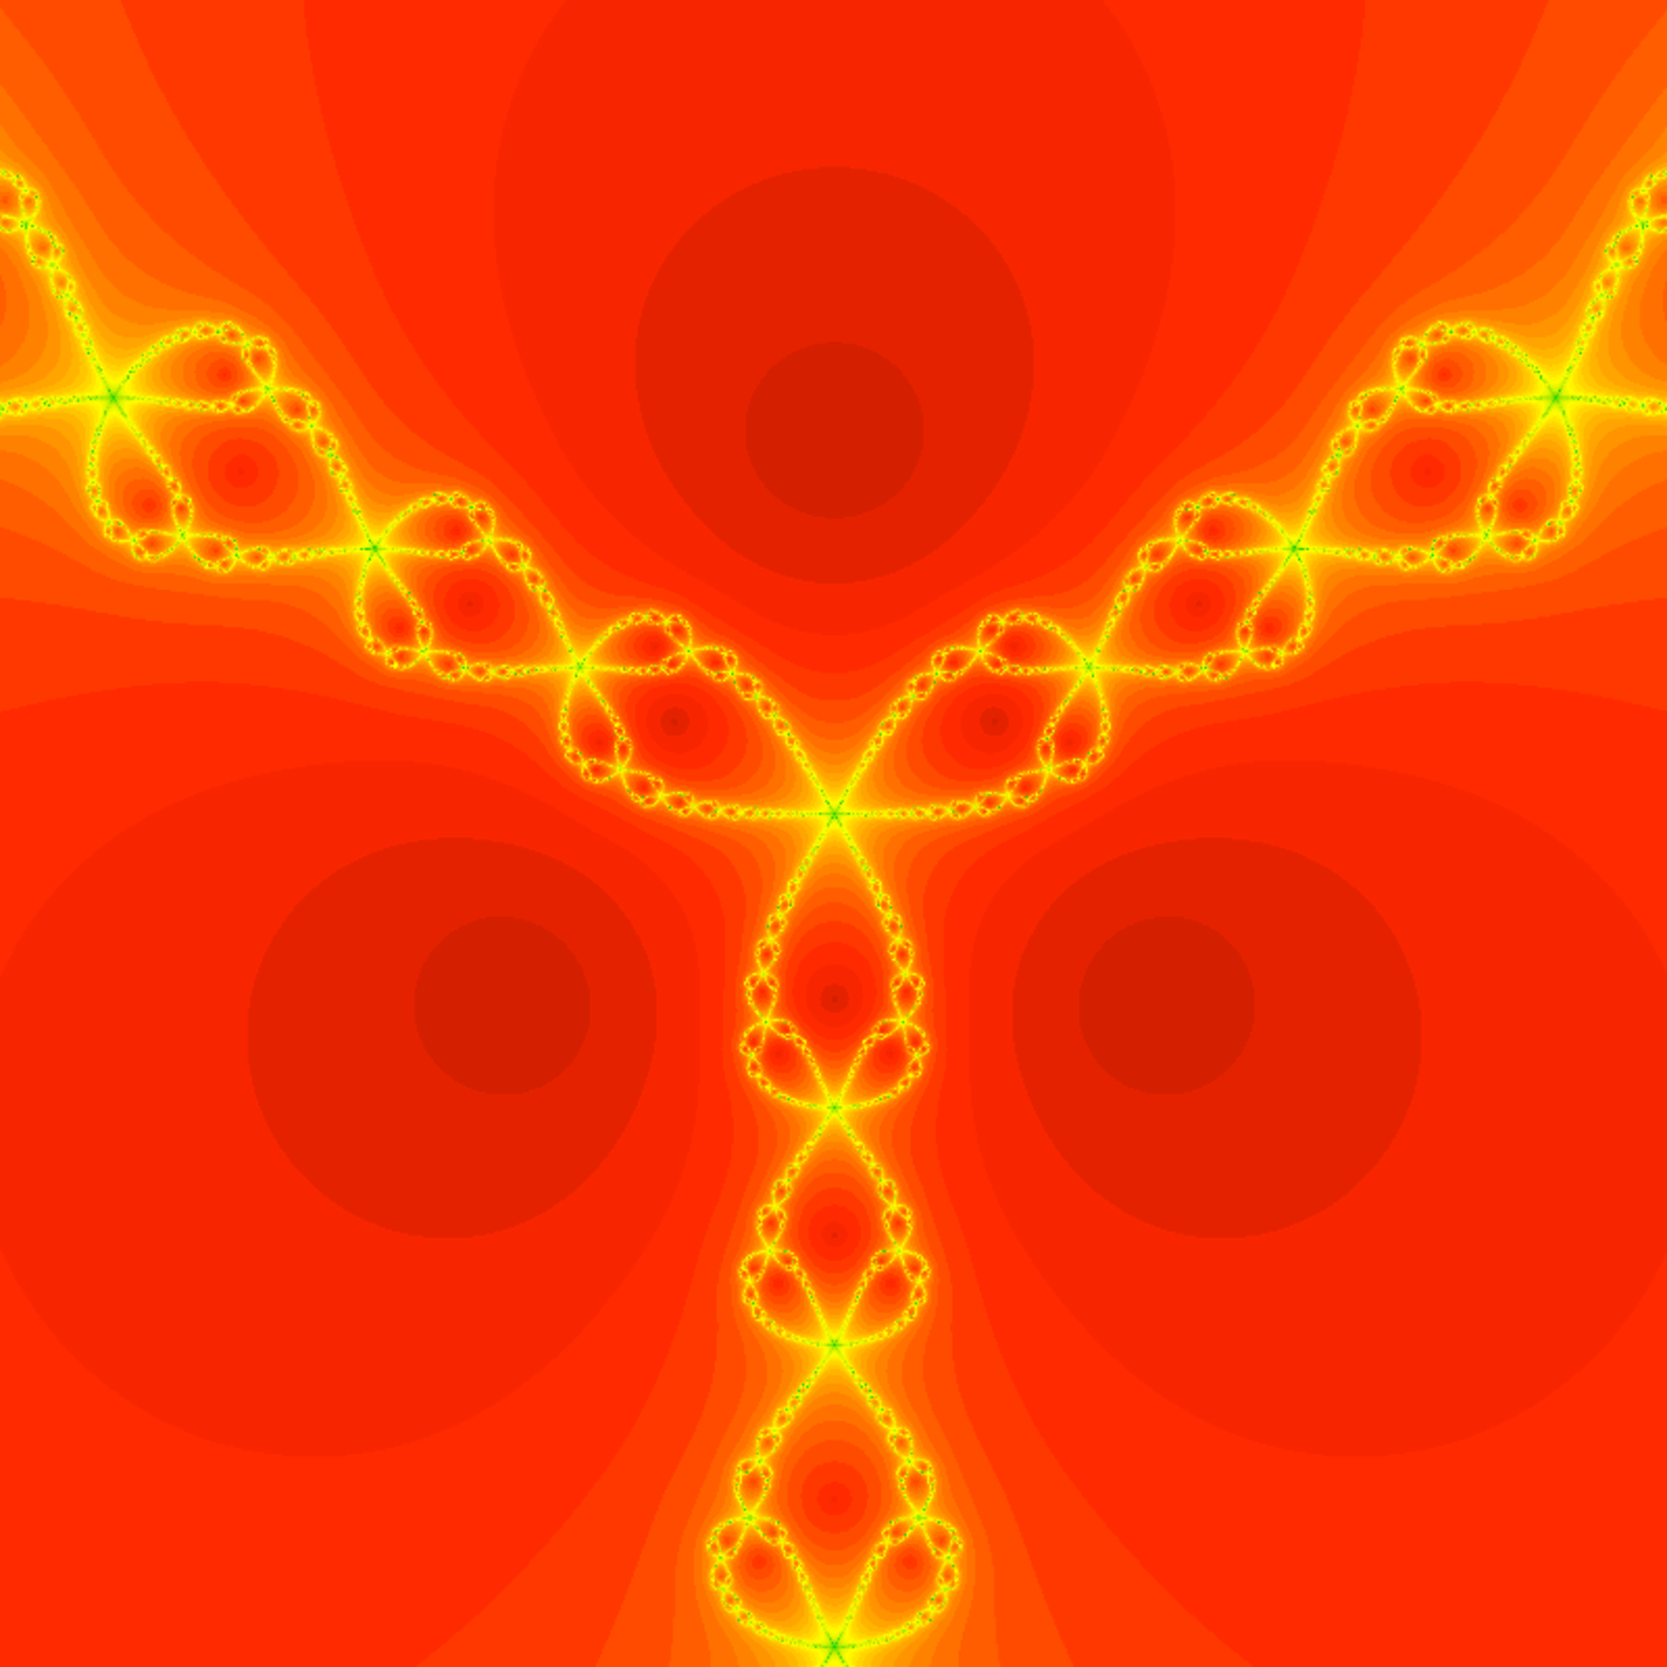
\includegraphics[width=6cm]{samplefigure.pdf}
\end{center}
\caption{\label{sample figure} \small The caption of this figure is ``Newton's method of a cubic polynomial".}
\end{figure}

%%%%%%%%
\section{Mathematics and packages} \label{packages}

By default, the following packages are uploaded:
\begin{enumerate}[\bf (1)]
\item {\tt enumerate:} It allows you to make list with specific somehow arbitrary labels, like this one.
\item {\tt amsthm:} To make evironments with different styles.
\item {\tt amsmath,amssymb,amsfonts:} Multiple mathematics symbols and fonts.
\item {\tt graphicx:} To include figures in a simple and intuitive way.
\item {\tt amscd:} To make commutative diagram with horizontal and vertical arrows. See below.
\item {\tt xy:} To make really fancy commutative arrows. See below.
\item {\tt booktabs:} To make fancy tables.
\end{enumerate}
You may add other standard packages if you need them but try to avoid it if at all possible.

If you need to use them, you will find information about these packages in the usual internet places. 

Here are examples of two commutative diagrams, one made with the package amscd and the other one with xy.

\[
\begin{CD}
A @>g>> B\\
@VV\pi V @VV\pi V\\
X @>f>> Y
\end{CD}
\]


\section{Bibliography}

You may include your references by hand using {\tt the bibliography} (see an example below) or, alternatively, you may use a .bib file and use BibTeX. In any case, we ask you to use a reasonable {\bf consistent} format for all your references. Our recommendation is using BibTex with the style   "plain" or "amsalpha".

%\newpage

\bibliography{fom_bib}{}
\bibliographystyle{plain}

%______________________________________________________________
\appendix
\vfill\newpage \section{Title of the appendix}
You can include here an appendix with details that can not be included in the core of the document. You should reference the sections in this appendix in the core document.
\vfill\newpage \section{Title of the appendix}
Second appendix.

\end{document}


